% Activate the following line by filling in the right side. If for example the name of the root file is Main.tex, write
% "...root = Main.tex" if the chapter file is in the same directory, and "...root = ../Main.tex" if the chapter is in a subdirectory.
 
%!TEX root =  dissertation.tex

\chapter[Appendix: Survey Response]{Appendix: Survey Response}\label{app:feedback}



\vspace{0.5cm}

\noindent%
\begin{minipage}{\linewidth}% to keep image and caption on one page
\makebox[\linewidth]{
  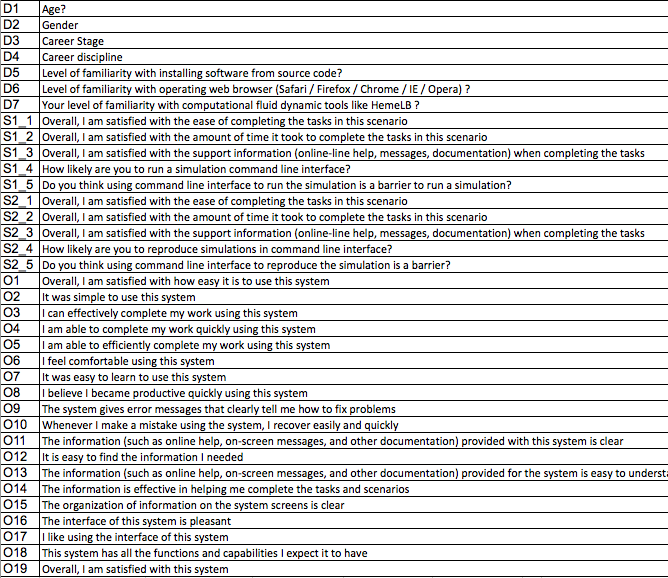
\includegraphics[keepaspectratio=true,scale=0.7]{../resources/evaluation/usability/raw0.png}
 }
\captionof{figure}{Survey response Question code} \label{fig:survey-response-0}%      only if needed  
\end{minipage}

\vspace{0.5cm}

\vspace{0.5cm}

\noindent%
\begin{minipage}{\linewidth}% to keep image and caption on one page
\makebox[\linewidth]{
  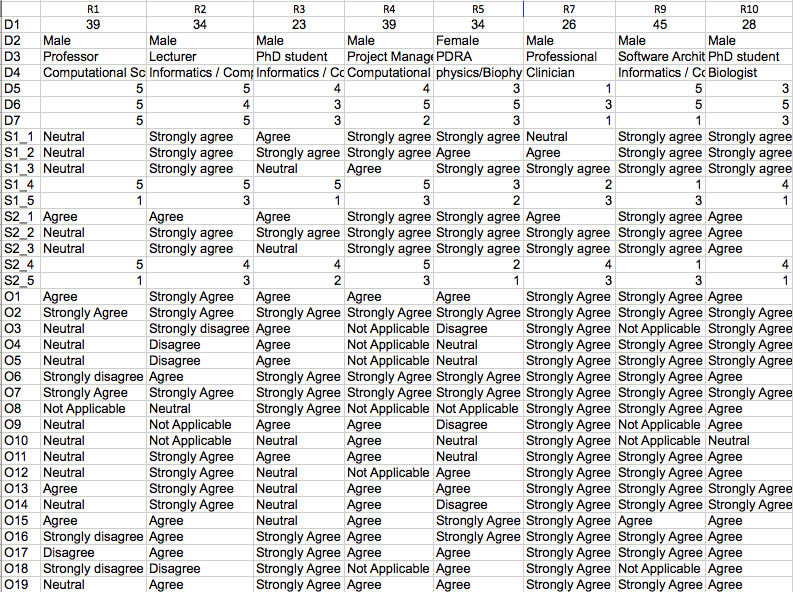
\includegraphics[keepaspectratio=true,scale=0.5]{../resources/evaluation/usability/raw1.png}
 }
\captionof{figure}{Survey response part 1} \label{fig:survey-response-1}%      only if needed  
\end{minipage}

\vspace{0.5cm}

\noindent%
\begin{minipage}{\linewidth}% to keep image and caption on one page
\makebox[\linewidth]{
  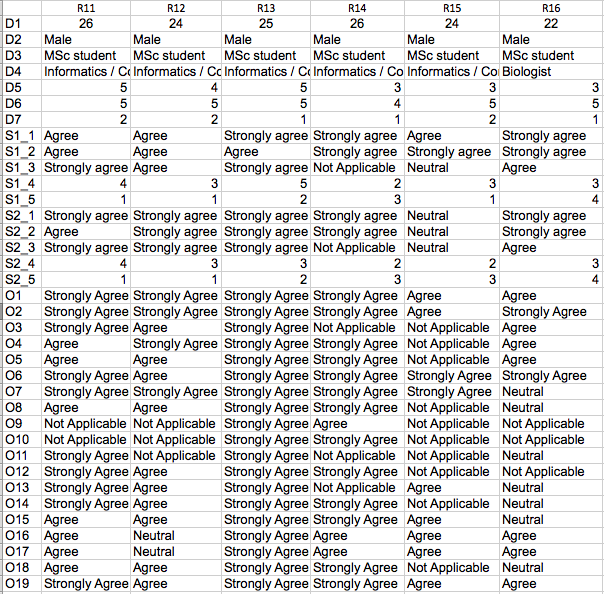
\includegraphics[keepaspectratio=true,scale=0.5]{../resources/evaluation/usability/raw2.png}
 }
\captionof{figure}{Survey response part 2} \label{fig:survey-response-2}%      only if needed  
\end{minipage}

\vspace{0.5cm}

\noindent%
\begin{minipage}{\linewidth}% to keep image and caption on one page
\makebox[\linewidth]{
  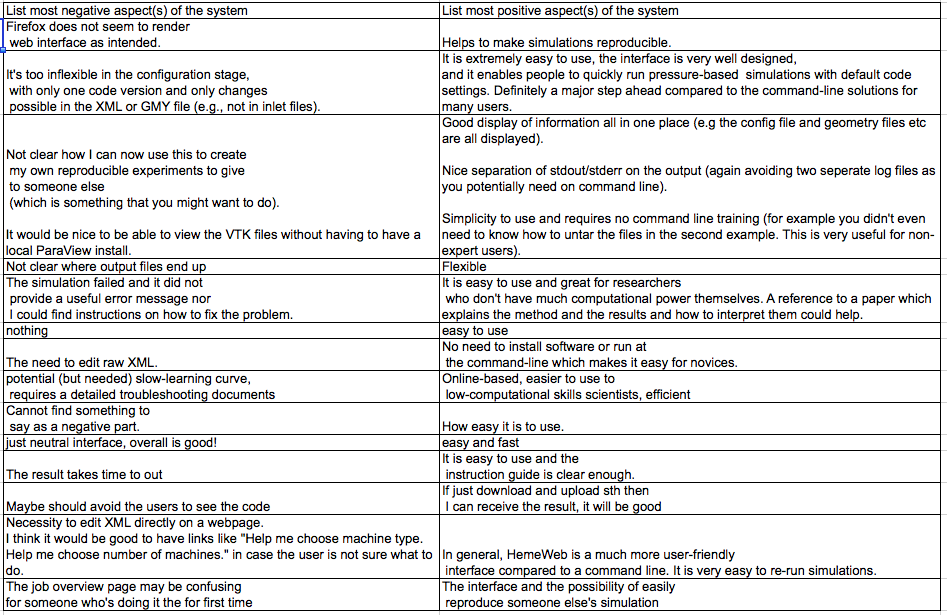
\includegraphics[keepaspectratio=true,scale=0.5]{../resources/evaluation/usability/feedback.png}
 }
\captionof{figure}{Survey response feedback} \label{fig:survey-feedback}%      only if needed  
\end{minipage}

\vspace{0.5cm}